\documentclass[12pt,a4paper]{article}
%\documentclass[8pt]{beamer}
%\usetheme{default}
%\usepackage[font=small,format=plain,labelfont=bf,up,textfont=it,up]{caption}
\usepackage{setspace}
\usepackage{graphicx}
\usepackage{epstopdf}
%\usepackage{natbib}
%\usepackage[num,overcite]{abntex2cite}
\usepackage{color}
%\usepackage{hyperref}
\usepackage[hidelinks]{hyperref}
\usepackage[alf]{abntex2cite}
%\citebrackets[]

%\bibpunct{(}{)}{;}{a}{}{,}
\usepackage[brazil]{babel}
\usepackage[utf8]{inputenc}
\usepackage {enumerate}
\usepackage{latexsym}
\usepackage{amsmath}
\usepackage{amsthm}
%\usepackage[T1]{fontenc}
%\usepackage{fetamont}
%\usepackage[num]{abntcite}
\usepackage{ mathrsfs }
\usepackage{subfigure}

%\setcitestyle{aysep={,}} 

\newcommand{\farcm}{\mbox{\ensuremath{.\mkern-4mu^\prime}}}%
\newcommand{\farcs}{\mbox{\ensuremath{.\!\!^{\prime\prime}}}}
\newcommand{\ii }{\'{\i}}
\newcommand{\cc }{\c c}
\newcommand{\cca}{\c ca }
\newcommand{\ao}{\~ao }
\newcommand{\cao}{\c c\~ao }
\newcommand{\oes}{\~oes }
\newcommand{\coes}{\c c\~oes }
\newcommand{\eq}{\begin{equation}}
\newcommand{\feq}{\end{equation}}
\newcommand{\dm}{\begin{displaymath}}
\newcommand{\fdm}{\end{displaymath}}
\newcommand{\eqn}{\begin{eqnarray}}
\newcommand{\feqn}{\end{eqnarray}}
\newcommand{\grau}{^{\circ}}
\newcommand{\ba}{\arrowvert_{t_1}^{t_2}}
\newcommand{\bc}{\arrowvert_{0^{\circ} {\rm C}}^{t_2}}
\newcommand{\bb}{\arrowvert_{0^{\circ} {\rm C}}^{t_1}}
\newcommand{\Ms}{$\mathrm{M}_{\odot}$}
%\renewcommand{\labelitemiv}{$-$}
\usepackage{amssymb}
\newcommand{\reg}[1]{#1$^{\tiny{\circledR}}$}
%\usepackage[hmargin=2cm,vmargin=2.5cm,bmargin=2cm]{geometry}
\usepackage[top=3cm, bottom=2cm, left=3cm, right=2cm,asymmetric]{geometry} 
\renewcommand{\baselinestretch}{1.5}

\usepackage{times}

\usepackage{float}

%Arial
%\usepackage{helvet}
%\renewcommand{\familydefault}{\sfdefault}

%Times New Roman
%\usepackage{mathptmx}

%\topmargin -1.5cm
%\leftmargin -2cm
%\rightmargin -2cm
%\oddsidemargin -0.7cm
%\textwidth 16cm
%\textheight 24cm
%\hoffset -1cm 

\usepackage{chngcntr}
%\counterwithout{figure}{chapter}

%\usepackage{fancyhdr}
%
%\fancypagestyle{mypagestyle}{
%\fancyhf{}
%\renewcommand{\headrulewidth}{0.5pt}
%
%\fancyhead[EL]{\normalsize \textsl{\nouppercase{\rightmark}}}
%\fancyhead[OL]{\normalsize \textsl{\nouppercase{\leftmark}}}
%\fancyhead[OR,ER]{}
%\cfoot{\thepage}
%}
%
%%\pagestyle{mypagestyle}

\usepackage[portuguese, boxed, ruled]{algorithm2e}
\usepackage{algorithmic}

\newtheorem{theorem}{Teorema}[section]
\newtheorem{definition}{Definição}[section]
%\newtheorem{lemma}{Lema}[chapter]
%\newtheorem{remark}{Observação}[chapter]

\renewcommand{\qedsymbol}{$\blacksquare$}

\usepackage{epic}
\usepackage{arydshln}
\providecommand{\sin}{} \renewcommand{\sin}{\hspace{2pt}\mathrm{sen}}
\numberwithin{equation}{section}
\usepackage{chngcntr}
%\counterwithout{equation}{section} % undo numbering system provided by phstyle.cls
%\counterwithin{equation}{chapter}
\counterwithin{table}{section}

\usepackage{multirow}
\usepackage{booktabs}

\setcounter{secnumdepth}{3}

\usepackage{tikz}
\usetikzlibrary{fit, shapes, arrows}
\usetikzlibrary{arrows.meta}
\usetikzlibrary{calc,patterns,angles,quotes}
\newcommand{\tikzMarkAngle}[3]{                                                
\tikzAngleOfLine#1#2{\AngleStart}                                              
\tikzAngleOfLine#1#3{\AngleEnd}                                                
\draw #1+(\AngleStart:0.15cm) arc (\AngleStart:\AngleEnd:0.15cm);              
}                                                                              


\tikzstyle{block} = [draw, fill=white, rectangle, 
    minimum height=3em, minimum width=6em, text width=2cm,align = center]
\tikzstyle{sum} = [draw, fill=white, circle, node distance=1cm]
\tikzstyle{input} = [coordinate]
\tikzstyle{output} = [coordinate]
\tikzstyle{pinstyle} = [pin edge={to-,thin,black}]

\tikzstyle{block1} = [draw, fill=white, rectangle, 
    minimum height=3em, minimum width=1em, text width=1cm,align = center]
\tikzstyle{sum} = [draw, fill=white, circle, node distance=1cm]
\tikzstyle{input} = [coordinate]
\tikzstyle{output} = [coordinate]
\tikzstyle{pinstyle} = [pin edge={to-,thin,black}]

\begin{document}
\pagenumbering{Roman}
% CAPA

\thispagestyle{empty}
\hspace{-1cm}
\begin{minipage}{0.35\textwidth}
%\begin{flushleft}
\vspace{-2cm}
  \begin{figure}[H]
    
\includegraphics[scale=0.07]{figures/UFMG-logo.png}
  \end{figure}
%\end{flushleft}  
\end{minipage}
\begin{minipage}{0.7\textwidth}
\textbf{UNIVERSIDADE FEDERAL DE MINAS GERAIS} \\
\textbf{PROGRAMA DE PÓS-GRADUAÇÃO EM ENGENHARIA ELÉTRICA}\\
\end{minipage}


\vspace{40mm}
\begin{center}
\textbf{
LUIZ ALBERTO QUEIROZ CORDOVIL JÚNIOR \\
RODRIGO FARIAS ARAÚJO}
\end{center}

\vspace{50 mm}
\begin{center}
\textbf{SISTEMAS NEBULOSOS: EXERCÍCIO COMPUTACIONAL 3}\\
\end{center}

\vspace{85mm}

\begin{center}
\textbf{Belo Horizonte - MG, 2017}
\end{center}
\thispagestyle{empty}
\newpage

%CONTRA-CAPA

\thispagestyle{empty}

\vspace{3 mm}
\begin{center}
\textbf{
LUIZ ALBERTO QUEIROZ CORDOVIL JÚNIOR \\
RODRIGO FARIAS ARAÚJO}
\end{center}

\vspace{35 mm}
\begin{center}
\textbf{APLICAÇÃO DO ALGORITMO C-MEANS PARA SEGMENTAÇÃO DE IMAGENS}\\
\end{center}

\vspace{30 mm}

\vspace{35mm}
\hspace{8cm}\begin{minipage}[r]{0.45\linewidth}
Relatório apresentado como requisito parcial para obtenção de aprovação na disciplina Sistemas Nebulosos do Programa de Pós-Graduação em Engenharia Elétrica, na Universidade Federal de Minas Gerais.\\ 
\\
Prof. Dr. André Paim Lemos
\end{minipage}

\vspace{50mm}
\begin{center}
\textbf{Belo Horizonte - MG, 2017}
\end{center}

\thispagestyle{empty}
\newpage
\tableofcontents
\newpage
\listoffigures
%\newpage
%\listoftables
\newpage
\pagenumbering{arabic}

%\documentclass[12pt,a4paper]{article}
%%\documentclass[8pt]{beamer}
%%\usetheme{default}
%%\usepackage[font=small,format=plain,labelfont=bf,up,textfont=it,up]{caption}
%%\usepackage{setspace}
%\usepackage{graphicx}
%\usepackage{epstopdf}
%\usepackage{natbib}
%\bibpunct{(}{)}{;}{a}{}{,}
%\usepackage[brazil]{babel}
%\usepackage[utf8]{inputenc}
%\usepackage {enumerate}
%\usepackage{latexsym}
%\usepackage{amsmath}
%%\usepackage[T1]{fontenc}
%%\usepackage{fetamont}
%%\usepackage[num]{abntcite}
%\usepackage{ mathrsfs }
%\usepackage{subfigure}
%\usepackage{helvet}
%\renewcommand{\familydefault}{\sfdefault}
%
%\newcommand{\farcm}{\mbox{\ensuremath{.\mkern-4mu^\prime}}}%
%\newcommand{\farcs}{\mbox{\ensuremath{.\!\!^{\prime\prime}}}}
%\newcommand{\ii }{\'{\i}}
%\newcommand{\cc }{\c c}
%\newcommand{\cca}{\c ca }
%\newcommand{\ao}{\~ao }
%\newcommand{\cao}{\c c\~ao }
%\newcommand{\oes}{\~oes }
%\newcommand{\coes}{\c c\~oes }
%\newcommand{\eq}{\begin{equation}}
%\newcommand{\feq}{\end{equation}}
%\newcommand{\dm}{\begin{displaymath}}
%\newcommand{\fdm}{\end{displaymath}}
%\newcommand{\eqn}{\begin{eqnarray}}
%\newcommand{\feqn}{\end{eqnarray}}
%\newcommand{\grau}{^{\circ}}
%\newcommand{\ba}{\arrowvert_{t_1}^{t_2}}
%\newcommand{\bc}{\arrowvert_{0^{\circ} {\rm C}}^{t_2}}
%\newcommand{\bb}{\arrowvert_{0^{\circ} {\rm C}}^{t_1}}
%\newcommand{\Ms}{$\mathrm{M}_{\odot}$}
%%\renewcommand{\labelitemiv}{$-$}
%\usepackage{amssymb}
%\newcommand{\reg}[1]{#1$^{\tiny{\circledR}}$}
%\usepackage[top=3cm, bottom=2cm, left=3cm, right=2cm,asymmetric]{geometry} 
%\renewcommand{\baselinestretch}{1.5}
%%\topmargin -1.5cm
%%\leftmargin -2cm
%%\rightmargin -2cm
%%\oddsidemargin -0.7cm
%%\textwidth 16cm
%%\textheight 24cm
%%\hoffset -1cm 
%
%\usepackage{epic}
%\usepackage{arydshln}
%\providecommand{\sin}{} \renewcommand{\sin}{\hspace{2pt}\mathrm{sen}}
%\numberwithin{equation}{section}

\section{Introdução}
Um algoritmo de agrupamento organiza itens em grupos, baseado no critério de similaridade. O algoritmo \textit{fuzzy c-Means} realiza agrupamentos de tal forma que determinado dado possuiu um grau de pertinência em relação a cada grupo, de modo que um maior grau de pertinência representa um maior compatibilidade do dado com o respectivo grupo, \textit{cluster}. 

\textit{Fuzzy c-Means}, é um algoritmo para análise de agrupamentos associado à representação de uma classe ou grupo singular em um dado conjunto de dados. Considerada como uma técnica de aprendizado não-supervisionado e raciocínio aproximado, possui aplicações diversas em tratativas de classificação de dados, dentre as quais aplicação à tarefa de classificação dados e segmentação de imagens abordadas neste trabalho.

% \textit{c} agrupamentos são representados por um vetor de centros \textit{C}.

<<<<<<< HEAD
O  Para que se alcance objetivo , realiza-se determinado número de iterações no sentido de minimizar a função de custo $J_{c}M(\mu_{h},C)$, em termos da distância euclidiana entre um ponto aleatório de um conjunto de dados e outro ponto, também aleatório, dito pertencente ao vetor de centros. 
=======
Para que se alcance o objetivo da \textit{clusterização}, realiza-se determinado número de iterações no sentido de minimizar a função de custo $J_{c}(\mu_{h},C)$, em termos da distância euclidiana entre um ponto aleatório de um conjunto de dados e outro ponto, também aleatório, dito pertencente ao vetor de centros. 
>>>>>>> 2d89d6191a861de75f52c44b082b8afe2d8f4b00

\begin{equation}
J=\sum_{i=1}^{N}\sum_{j=1}^{C}\mu_{ij}^{m}\lVert x_{i}-c_{j} \rVert^2
\end{equation}

onde:
\begin{itemize}
	\item $N$: número de dados;
	\item $\mathcal{C}$: número de grupos (\textit{clusters});
	\item $c_{j}$: centro do $j$-ésimo grupo;
	\item $\mu_{ij}$: grau de pertinência do $i$-ésimo dado $x_{i}$ em relação ao $j$-ésimo grupo.
\end{itemize}

A norma, $\lVert x_{i}-c_{j} \rVert$, mede a similaridade (ou proximidade) de um dado elemento $x_{i}$ para vetor de centro $c_{j}$ do \textit{j}. Para cada ponto $x_{i}$, o grau de pertinência para cada $c_{j}$ é calculado da seguinte forma:

%Em cada iteração, o algoritmo mantém o vetor centro para cada \textit{cluster}. 

\begin{equation}
\mu_{ij}=\frac{1}{\sum_{k=1}^{C}(\frac{\lVert x_{i}-c_{j} \rVert}{\lVert x_{i}-c_{k} \rVert})^\frac{2}{m-1}}
\end{equation}
onde \textit{m} é coeficiente de fuzzificação.

Cada centro $c_{j}$ é calculado como:

\begin{equation}
c_{j}=\frac{\sum_{i=1}^{N}\mu_{ij}^m x_{i}}{\sum_{1}^{N}\mu_{ij}^m}
\end{equation}

No início do algoritmo, o grau de pertinência para os dados é inicializado com um valor randômico no intervalo $[0,1]$ tal que $\sum_{j}^{C}\mu_{ij}=1$.
O coeficiente de fuzzificação $m \in [1,\infty)$, mede a tolerância do grupo. Este valor determina o quanto um grupo pode sobrepor outro. Quanto maior este valor, maior a sobreposição entre os agrupamentos.

O critério de parada é expresso em termos da acurácia dos graus de pertinência aplicados ao conjunto de dados, no sentido de determinar o número de iterações durante o processo de minimização. Esta pode ser calculada utilizando a norma entre o vetor de centros, $C^k$ da $k$-ésima iteração, e o vetor $C^{k-1}$.

\begin{algorithm}[H]
	\textbf{Agrupamento}\\
	Determinar a quantidade de partições \textit{c}; \\
	Determinar o erro máximo $\epsilon$;\\
	Inicializar os centros aleatoriamente;\\
	Inicializar o contador de iterações $k=0$;\\
	\textbf{repita}\\
	Incrementar $k$;\\
	Atualizar $\mu_{h}$;\\
	Atualizar $C$;\\
	\textbf{até que} $\lVert C^{(t)}-C^{(t-1)} \rVert < \epsilon$
	\caption{Algoritmo Fuzzy c-Means}
\end{algorithm}

\section{Descrição do Experimentos}
\label{section:descr}

Com o objetivo de avaliar o algoritmo \textit{c-means} foram elaborados os seguintes experimentos:

\begin{enumerate}
	\item Aplicação do algoritmo \textit{fuzzy c-means} desenvolvido ao conjunto de dados \texttt{fcmdata.dat} para 4 (quatro) grupos de agrupamentos e comparação dos resultados obtidos com a função \texttt{fcm} do MATLAB.
	\item Adaptação do algoritmo anterior para o problema de segmentação de imagens e comparação dos resultados obtidos com a função \texttt{fcm} do MATLAB para o espaço de cores RGB utilizando diferentes quantidades de grupos de agrupamento.
	%(nesse exercício você deve escolher o número de grupos de acordo com sua avaliação da imagem).
\end{enumerate}

A Figura \ref{fig:fcmdata} e \ref{fig:images} ilustram os dados do conjunto \texttt{fcmdata.dat} e as imagens utilizadas na aplicação do algoritmo \textit{c-means} para segmentação de imagens, respectivamente.

\begin{figure}[ht!]
	\centering
	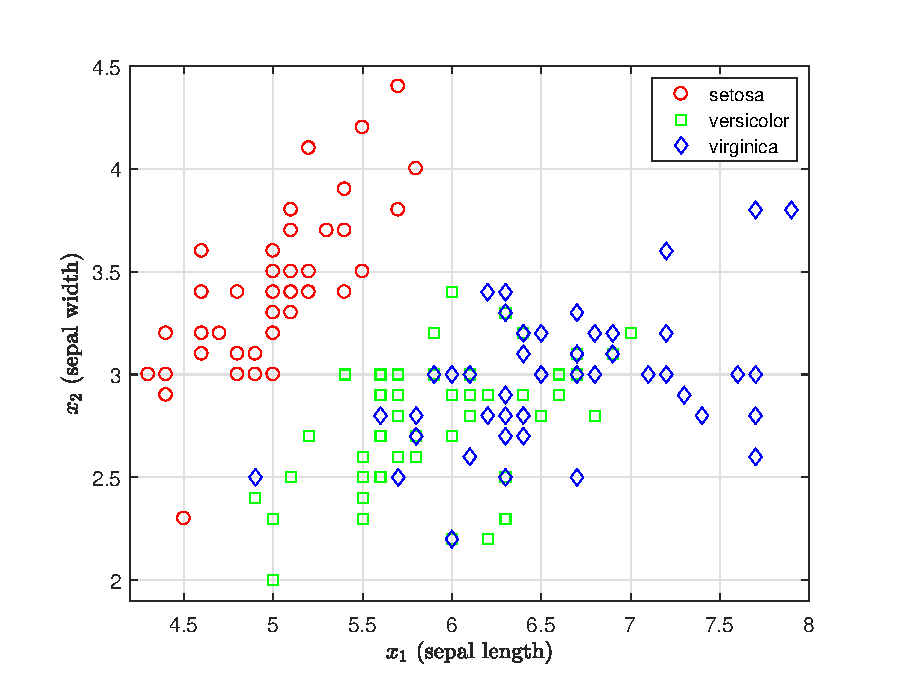
\includegraphics[width=0.7\textwidth]{figures/data.eps}
	\caption{Conjunto de dados \texttt{fcmdata.dat}.}
	\label{fig:fcmdata}
\end{figure}

\begin{figure}[!htbp]
	\centering
	\subfigure[Imagem $01$]{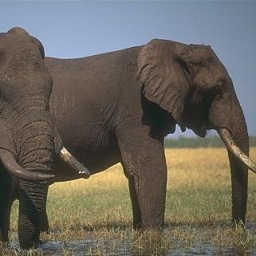
\includegraphics[width = 0.4\textwidth]{figures/img01.jpg}}
	\subfigure[Imagem $02$]{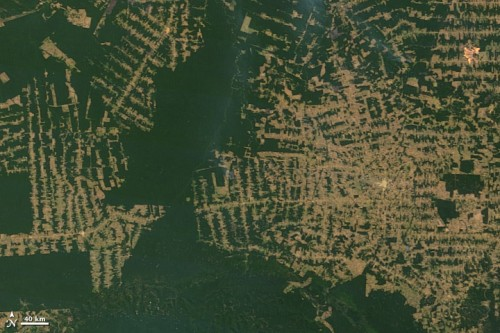
\includegraphics[width = 0.5\textwidth, height = 0.26\textheight]{figures/img02.jpg}}
	\subfigure[Imagem $03$]{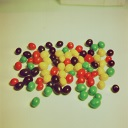
\includegraphics[width = 0.28\textwidth]{figures/img03.jpg}}
	\caption{Imagens usadas na aplicação do algoritmo c-means para segmentação de imagens.}
	\label{fig:images}
\end{figure}

%\subsection{Procedimentos Computacionais}
\section{Resultados} \label{sec:results}

Nesta seção serão apresentados os resultados dos experimentos descritos anteriormente na Seção \ref{section:descr}.

\subsection{Agrupamento de dados}

O algoritmo \textit{c-Means} implementado foi utilizado para agrupamento de elementos do conjunto de dados \textit{fcmdata.dat}, considerando 4 grupos. Nas Figuras \ref{fig:resul_cluster_cmeans} e \ref{fig:resul_cluster_fcm} são ilustrados os centros dos agrupamentos obtidos quando utilizado o algoritmo implementado e a função \texttt{fcm} do MATLAB, respectivamente.

\begin{figure}[!htbp]
	\centering
	\subfigure[Algoritmo desenvolvido.]{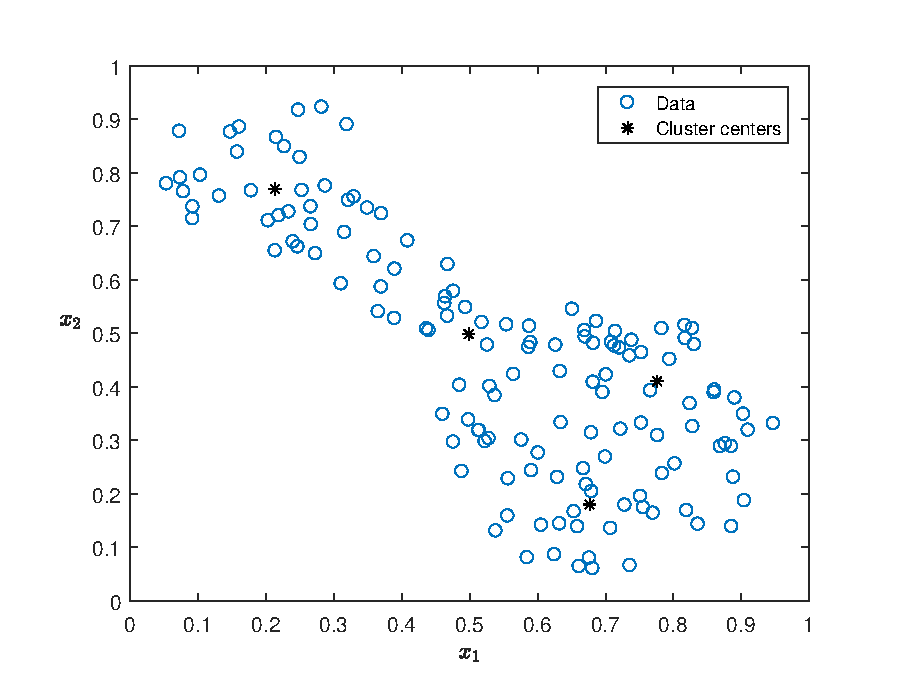
\includegraphics[width = 0.48\textwidth]{figures/data_cmeans.eps}\label{fig:resul_cluster_cmeans}}
	\subfigure[Função \texttt{fcm} do MATLAB.]{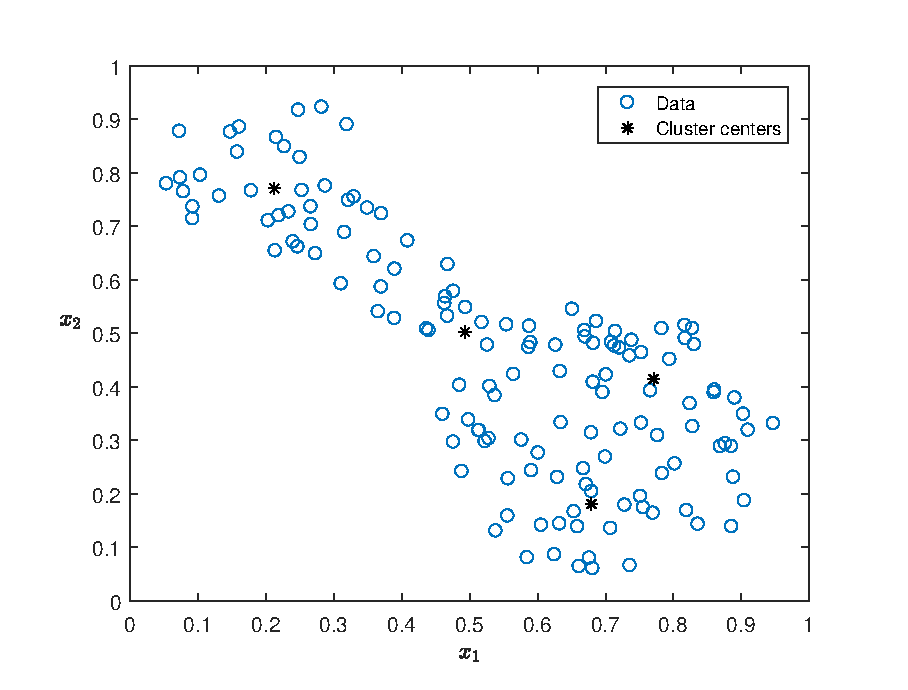
\includegraphics[width = 0.48\textwidth]{figures/data_fcm.eps}\label{fig:resul_cluster_fcm}}
	\caption{Comparação dos centros dos agrupamentos, considerando 4 agrupamentos, obtidos por meio do algoritmo c-means implementado e da função \texttt{fcm} do MATLAB.}
\end{figure}

\subsection{Segmentação de imagens}
\label{subsection:seg}

Na abordagem computacional, por meio da técnica de validação cruzada, cada conjunto de espécies foi separado de forma aleatória em subconjuntos de treinamento e validação representados, com dimensão de $70\%$ e $30\%$, respectivamente de cada classe de padrões.

Para todas as classes, no total, quatro dados de entrada aplicados a três espécies, com $50$ amostras. Como ferramenta de aprendizagem, os conjuntos de treinamento e validação, foram determinados observando-se os percentuais em $35$ e $15$ amostras, respectivamente, para cada classe $C_{j}$.

Neste sentido, na etapa de treinamento, a partir de aprendizado supervisionado, houve a classificação inicial das amostras, como função da quantidade de regras e dos graus de certeza, no sentido de se estabelecer as condições e parâmetros iniciais do sistema de classificação.

A partir destes, houve a implementação das características de contexto adquiridas na etapa de treinamento, no sentido de aferir-se o desempenho do sistema de classificação.

Os experimentos foram realizados $25$ vezes, para cada número de funções de pertinência de $2$ até $15$, com o propósito de se observar o limiar de convergência e paridade entre o erro do conjunto de treinamento e erro no conjunto de validação e eliminar a natureza estocástica da escolha do dados de treinamento de validação.

Nota-se que, para ambas as \textit{t-normas} o número dito ideal de funções de pertinência é $8$. De modo que, para um número menor de funções de pertinência ocorre o chamado \textit{underfitting}, e para um número maior de funções de pertinência ocorre o chamado \textit{overfitting}.

%As amostras foram escolhidas aleatoriamente dentro dos subconjuntos e avaliadas para cada conjunto de regras, por n repetidas vezes.

\newpage
\section{Conclusões}

A utilização de métodos de classificação oferece uma solução baseada em conhecimento adquirido por aprendizagem ativa. Nesta abordagem, a classificação de pontos afins com relação aos seus respectivos centros, é relevante para análise de similaridade entre conjuntos de dados não-rotulados. 

Com a aplicação de algoritmo \textit{fuzzy c-Means} observou-se na realização dos experimentos, o efeito da aplicação das relações nebulosas e avaliação baseada em acurácia, em processos de inferência, propiciando distinção entre os dados de acordo com suas características de contexto.

Nos experimentos de segmentação de imagem e no agrupamento de um conjunto de dados não-rotulados, a rotina implementada apresentou resultado bastante similar tomando-se como referência a função \texttt{fcm} do MATLAB\textcopyright, apresentado desempenho satisfatório, conforme indicado na Seção \ref{sec:results}.

\newpage

\section*{Referências}
\addcontentsline{toc}{section}{\protect\numberline{}Referências}%

\noindent [1] COUTINHO, P. H. S. Proposta de Novos Algoritmos Híbridos de Clusterização Fuzzy e suas aplicações. Trabalho de Conclusão de Curso. Departamento de Ciências Exatas e Tecnológicas. Universidade Estadual de Santa Cruz. Ilhéus-Bahia, 2017.

[2] CANNON, Robert L.; DAVE, Jitendra V.; BEZDEK, James C. Efficient implementation of the fuzzy c-means clustering algorithms. IEEE transactions on pattern analysis and machine intelligence, n. 2, p. 248-255, 1986.

\end{document}
